\epigraph{\textit{Information flow is what the Internet is about. Information sharing is power. If you don't share your ideas, smart people can't do anything about them, and you'll remain anonymous and powerless.}}{-- \textup{Vint Cerf}}

We have seen thus far the two main export formats supported by Wikidata, namely, RDF and JSON. However, none of them are suitable for analytical queries. In this chapter, we will explore the possibility of exporting Wikidata in a columnar format, as we have mentioned in the previous chapter, DuckDB is the perfect candidate for this task. This is, we will create a Rust-based solution for exporting Wikidata to DuckDB.

\section{The issue with JSON and other text-based formats}
\label{section:issue}

JSON is a text-based format, and as such, the data that is stored inside a JSON file is not compressed in any way. This means that the size of the file is directly proportional to the size of the data. This is not a problem for small datasets, but it becomes an issue when we are dealing with larger information repositories. As we have seen in the introductory chapter a Wikidata JSON dump is around \texttt{1.5 TB} in size when uncompressed. See Chapter \ref{chapter:intro} for a more detailed explanation. The challenge lies in the inability to load such a massive file into the memory of a single machine. Even if feasible, the loading process would be time-consuming and incur substantial expenses for renting a suitable machine. As a result, a binary format is required to store the information. This is where DuckDB comes into play. Despite the need to load the database into memory (recall, DuckDB is an in-process or embedded database), the repository's size is considerably smaller than that of the JSON file, often differing by several orders of magnitude. DuckDB achieves this by utilizing a columnar database structure, enabling more efficient compression of the data compared to a text-based format. This compression advantage is the primary reason driving our decision to export Wikidata to DuckDB.

It is worth mentioning that Wikidata JSON dumps follow a structure where each line of the file stores a single object. This provides the advantage of being able to parse the file line by line, which is quite convenient. However, there is a drawback: every line in the dump includes redundant boilerplate information related to the JSON object schema. In other words, we may have hundreds of millions of lines, all containing the same boilerplate code. Instead of having a header with the object schema, it is repeated in every line of the document. This redundancy significantly impacts the memory efficiency of JSON files. While JSON is excellent for sharing information, it is not the most efficient option for storage purposes.

\section{wd2duckdb}

Now that we have a clear understanding of the scope of the project, we can start working on the design of the tool in charge of transforming the Wikidata JSON dumps into a DuckDB file. For us to do so, some decisions are made. First, we are interested in storing only one of the translations of each Wikidata entity; that is, we are going to store only one of the labels, descriptions and aliases of each item. However, the language of choice can be modified\footnote{\url{https://github.com/angelip2303/wd2duckdb/blob/master/wikidata-rs/src/lib.rs\#L20}}. Second, we are going to store only the statements that are not deprecated. Apart from that, the rest of the information is going to be stored as it is.

\label{section:wd2duckdb_design}
\subsection{Design}

The tool is going to be divided into two main parts. The first one is going to be in charge of parsing the Wikidata JSON dump and extracting the information that we are interested in. The second part is going to be in charge of storing the information in a DuckDB database. The idea is to allow backends to be interchangeable; that is, several implementations for other drivers should be implemented without actually changing the existing code. However, for the sake of simplicity, we are going to focus on DuckDB for the time being.

\label{section:json_dump}
\subsubsection{Parsing the JSON dump}

The first part of the tool is going to be in charge of parsing the Wikidata JSON dump and extracting the information that we are interested in. In this manner, we are going to parse the JSON dump line by line. Recall, each line of the dump contains a single JSON object, which is -- indeed -- a Wikidata entity. It is worth noting that the entities in the array are not sorted in any way. This is, we have to be aware that the first entity in the dump is not necessarily the first Wikidata entity, namely, \texttt{Q1}. Thus, our solution should not rely on the order of the entities in the dump. What's more, a certain entity of the dump can refer to another that has not been parsed yet. Hence, we must be able to handle this situation as well.

Having that said, it is worth mentioning that a Wikidata dump can contain hundreds of millions of entities. This means that we cannot store all that information in memory. Hence, we must find a way to append the information to the resulting database as we parse the dump.

\label{section:duckdb_load}
\subsubsection{Storing the information in DuckDB}

The second part of the tool is going to be in charge of storing the information we have retrieved in the resulting database. Hence, we are going to load the following information into DuckDB:

\begin{itemize}
    \itemsep0.5em
    \item \textbf{Wikidata IDs}: As we had seen in section \ref{section:wikibase_graphs}, Wikidata IDs consist of a type prefix \texttt{Q}, \texttt{P} or \texttt{L}, for identifying Entities, Properties or Lexemes, followed by a sequence of numbers. There exist other two types of IDs, namely, \texttt{F} and \texttt{S}, for identifying Forms and Senses, respectively. A more detailed discussion on this topic will be presented later on.
    \item \textbf{Labels}: We are going to store the labels of the entities in the same table where we store the IDs.
    \item \textbf{Descriptions}: We are storing the descriptions of the entities in the same table where we store the IDs.
    \item \textbf{Statements}: We are going to store the statements of the entities in a separate table so that we can build the graph later on. The idea is to store the ID of the source entity, the ID of the property and the ID of the destination entity. In this manner, we will end up with two main tables: one for storing the entities, or vertices, and another one for storing the statements, or edges. Several other tables are going to be created for storing data relative to the information that comes with the statements, such as qualifiers, references, ranks, etc. However, for the time being, we are going to focus on the main tables.
\end{itemize}

According to what we have just described, we are going to end up with a database that contains two main tables: one for storing the entities, or vertices, and another one for storing the statements, or edges. The schema of the database is depicted in figure \ref{fig:schema}.

\begin{figure}[ht]
    \centering
    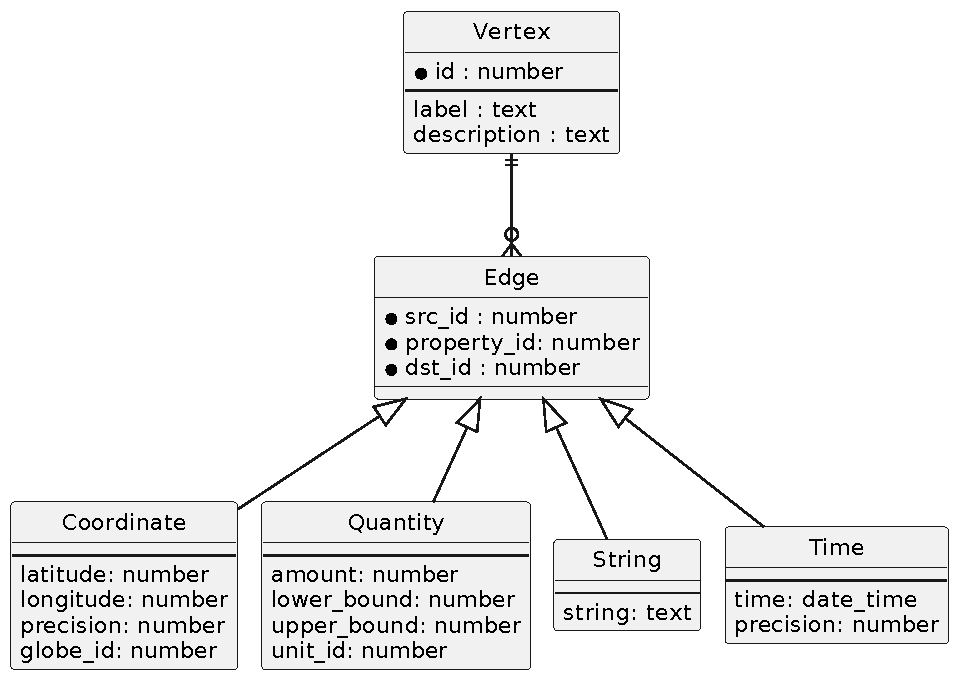
\includegraphics[width=.75\linewidth]{figures/diagrams/10-1_wd2duckdb.pdf}
    \caption{Entity-relationship diagram of the Database created by the \texttt{wd2duckdb} tool}
    \label{fig:schema}
\end{figure}%

\subsection{Implementation of the \texttt{wd2duckdb} tool}

Once we have a better understanding of the design of the tool. Now, we can start working on the implementation of it. The idea is to create a Rust-based solution that can be used as a library or as a command-line tool. This CLI will act as a wrapper for the library and is responsible for calling it, as well as handling command-line inputs such as the source JSON and the target file. Through \texttt{crates.io}\footnote{\url{https://crates.io/crates/wikidata-rs}}, we aim to make the library available to other Rust projects. This is, we are looking to decouple the library from the binary for other backends to be implemented on top of the same traits.

The most relevant aspect of the implementation revolves around the insertion of the processed Wikidata entities into the database. To accomplish this, we will leverage the powerful \texttt{duckdb-rs}\footnote{\url{https://crates.io/crates/duckdb}} library, which provides a Rust interface for DuckDB. Note that, it is based on the same interface as the SQLite driver for Rust. The plan is to utilize this library to create the necessary database and tables, and then employ it again to insert the data into it. The diagram in Figure \ref{fig:activity} illustrates the implementation of the \texttt{wd2duckdb} tool.

To insert the data into the database, we first need to establish a connection to it by creating a \texttt{Connection} object. Subsequently, we create the \texttt{Statement} and execute the corresponding SQL statement, specifically an insert one. However, the main concern arises executing the aforementioned statements for each entity, as it would severely impact the tool's performance due to the need for creating numerous connections to the database, corresponding to the number of lines in the JSON dump. To address this issue, we employ a transactional approach. By creating a transaction and executing the insert statements within it, we can greatly enhance the tool's performance. Once all the entities have been inserted, we commit the transaction. Notably, this approach requires only a single connection to the database. It becomes even more convenient when utilizing the \texttt{duckdb-rs} library, as it provides an \texttt{Appender} struct. The \texttt{Appender} not only encapsulates the transaction but also optimizes the data insertion process by buffering the data and inserting it into the database in batches. Consequently, the tool's performance is further improved. This is the recommended approach for inserting large amounts of data into a database.

\begin{figure}[p]
    \centering
    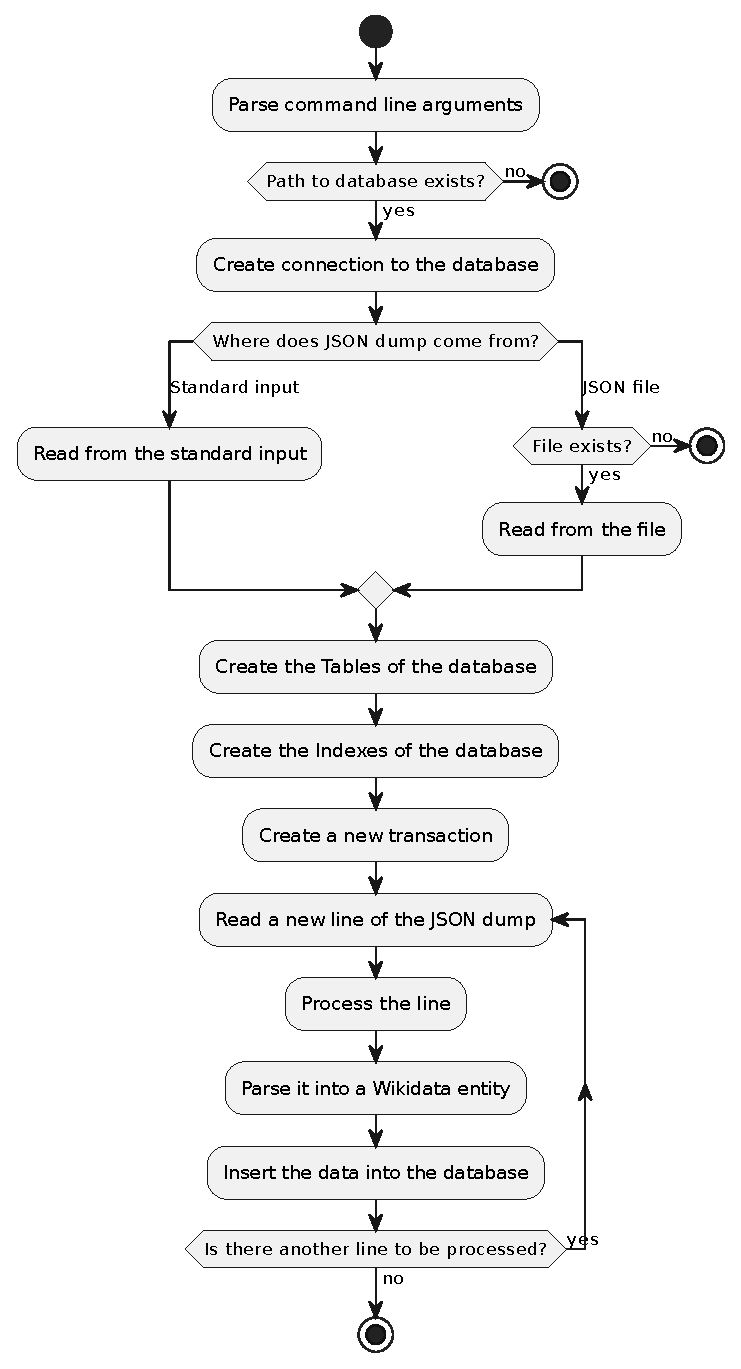
\includegraphics[width=.66\linewidth]{figures/diagrams/10-2_wd2duckdb.pdf}
    \caption{Activity diagram of the \texttt{wd2duckdb} tool}
    \label{fig:activity}
\end{figure}%

\subsection{Optimizations}

The Wikidata JSON dump is a huge file. As we have seen in section \ref{section:issue}, it is around \texttt{1.5 TB} in size. This means that we need to put an extra effort into optimizing the tool. For that, we are going to use a combination of different techniques, such as compression, and fine-tuning the chosen data types.

\subsubsection{Compression}

Dealing with large amounts of data is far from being trivial. For that, we are going to use compression techniques to reduce the size of the data that we are going to store. Those mechanisms can potentially reduce the size of the data by a factor of 10. This is not only beneficial for reducing the storage footprint, but it also helps improve the performance of tools consuming the data as fewer reads from disk or over a network connection are required. Column store formats are known for being highly compressible, and DuckDB is not an exception. This is because data within a column tends to be similar to each other, which is not the case for row-based formats, where each row is composed of heterogeneous data types, leading to lower compression rates.

The best thing about compression in DuckDB is that it will automatically choose the better compression algorithm for us \cite{Raasveldt_2022}. This is because it can detect the data type of each column, and based on that, it will choose the best compression method. For example, DuckDB will probably choose \texttt{RLE or Run-length encoding} for storing the identifiers of the properties, as it decomposes the dataset into pairs of (value, count) tuples, where the count represents how many times the value is repeated. Thus, no repeated values are stored. This is useful as several different entities may claim the same property, such as \texttt{P31} (instance of), where almost every Wikidata item will have it. Hence, we can take advantage of this and compress the data using \texttt{RLE}. To put it in a nutshell, \texttt{RLE} is a lossless compression algorithm that replaces repeated values with a single value and a count. This is illustrated in figure \ref{fig:rle}.

\begin{figure}[ht]
    \centering
    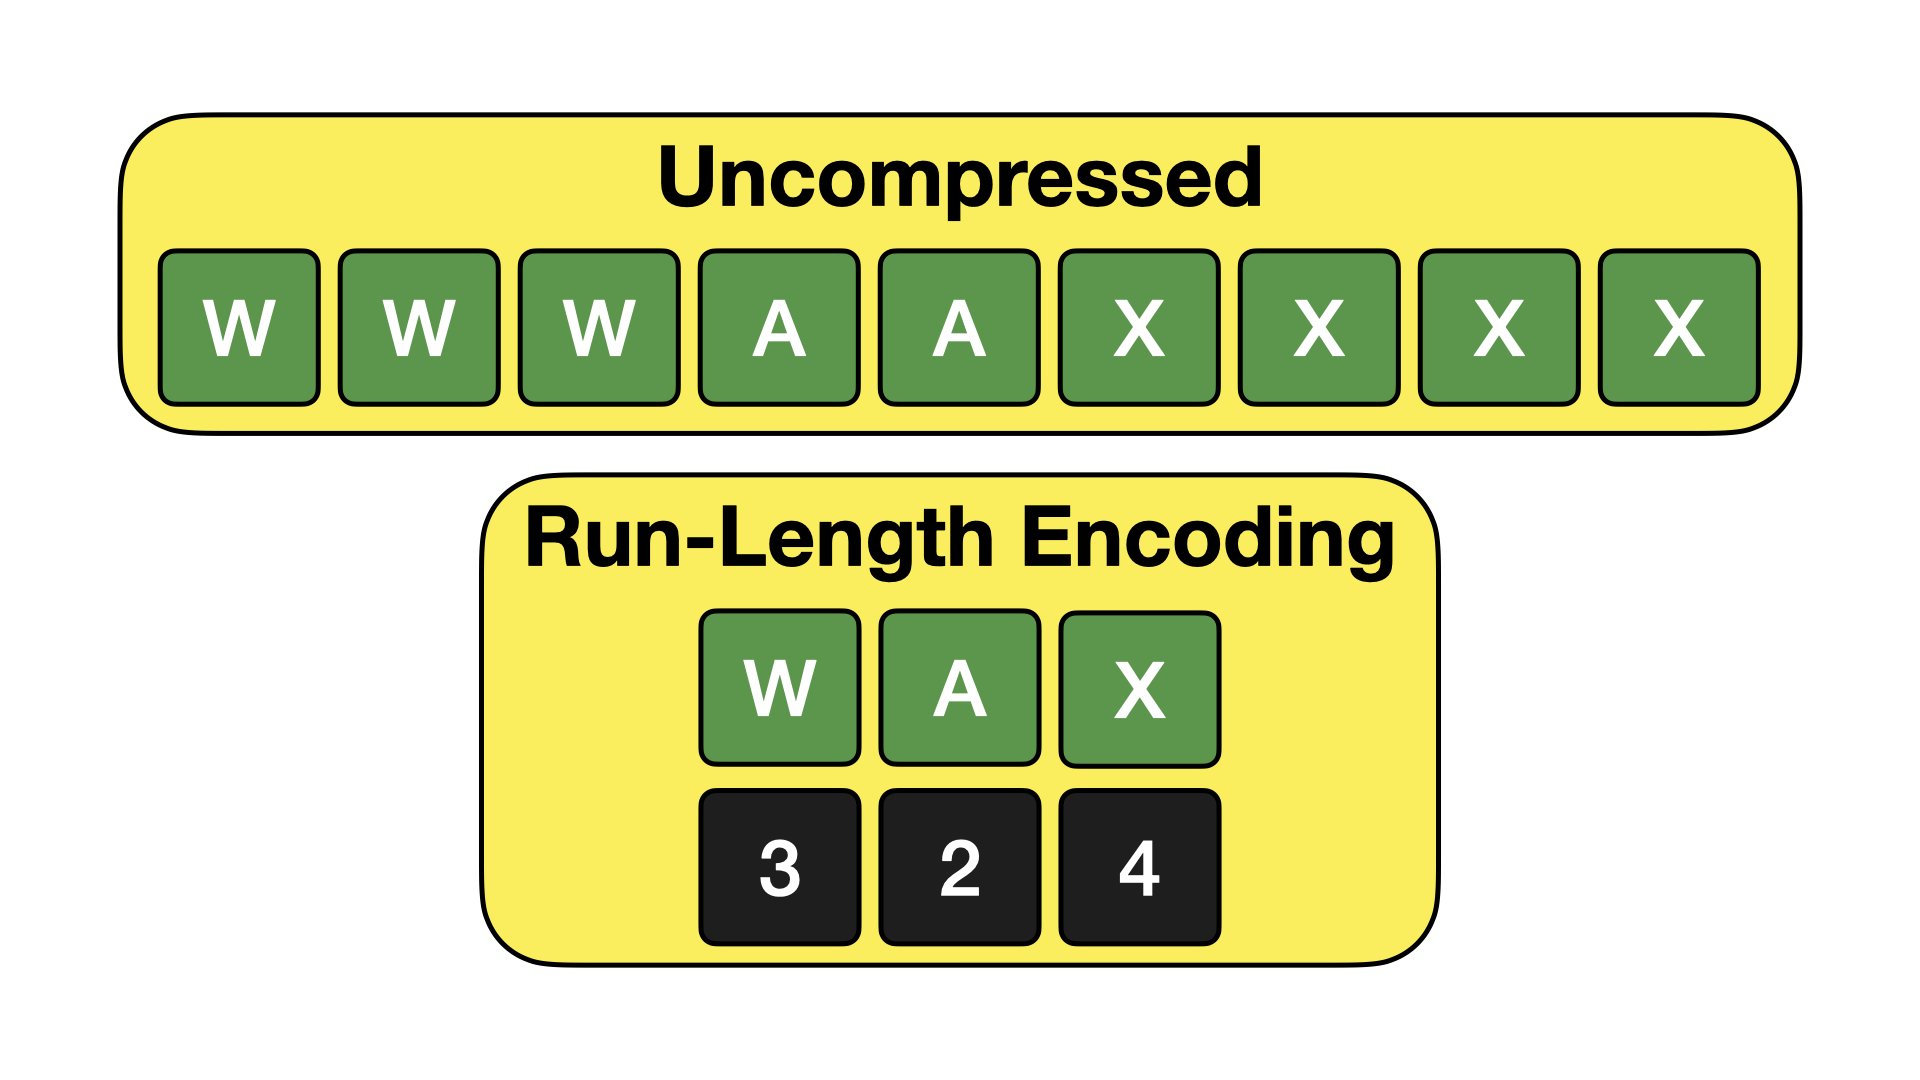
\includegraphics[width=.8\linewidth]{figures/diagrams/10-2_rle.png}
    \caption[Example of \texttt{RLE} compression]{Example of \texttt{RLE} compression \cite{Raasveldt_2022}}
    \label{fig:rle}
\end{figure}

In the given example, the original sequence \texttt{WWWAAXXXX} is compressed into \texttt{3W2A4X}. This transformation is achieved by identifying repeated characters, such as the \texttt{W} occurring thrice, the \texttt{A} occurring twice, and the \texttt{X} occurring four times. Thus, we can replace the repeated values with a single value and a count. The \textit{run-length encoding} preserves the same information as the original sequence but in a more concise format. Additionally, we have successfully represented the initial string, consisting of nine characters, with a string of only six characters, resulting in a 33\% reduction in size. It is worth noting that the compression rate improves as the number of repetitions increases. Although this example is straightforward, it effectively demonstrates the underlying concept of \texttt{RLE}.

Another possibility is \texttt{FSST or Fast Random Access String} for compressing \texttt{STRING} columns. This mechanism aims for creating a dictionary of references and segments which are repeated across the dataset. This is effective when dealing with unique strings, such as \textit{labels} or \textit{descriptions} in our case, having plenty of repetitions within them. For example, descriptions of entities from the same real-world domain may contain repeated words, such as in the case of \texttt{Q2} (Earth) or \texttt{Q193} (Saturn), where the word \texttt{planet} may appear several times. Thus, we can take advantage of this, and compress the data using the \texttt{FSST} algorithm. The way it works is by creating a \textit{symbol table} that maps each unique string to an integer identifier. Then, the original string is replaced by the corresponding identifier. This is illustrated in figure \ref{fig:fsst}.

\begin{figure}[ht]
    \centering
    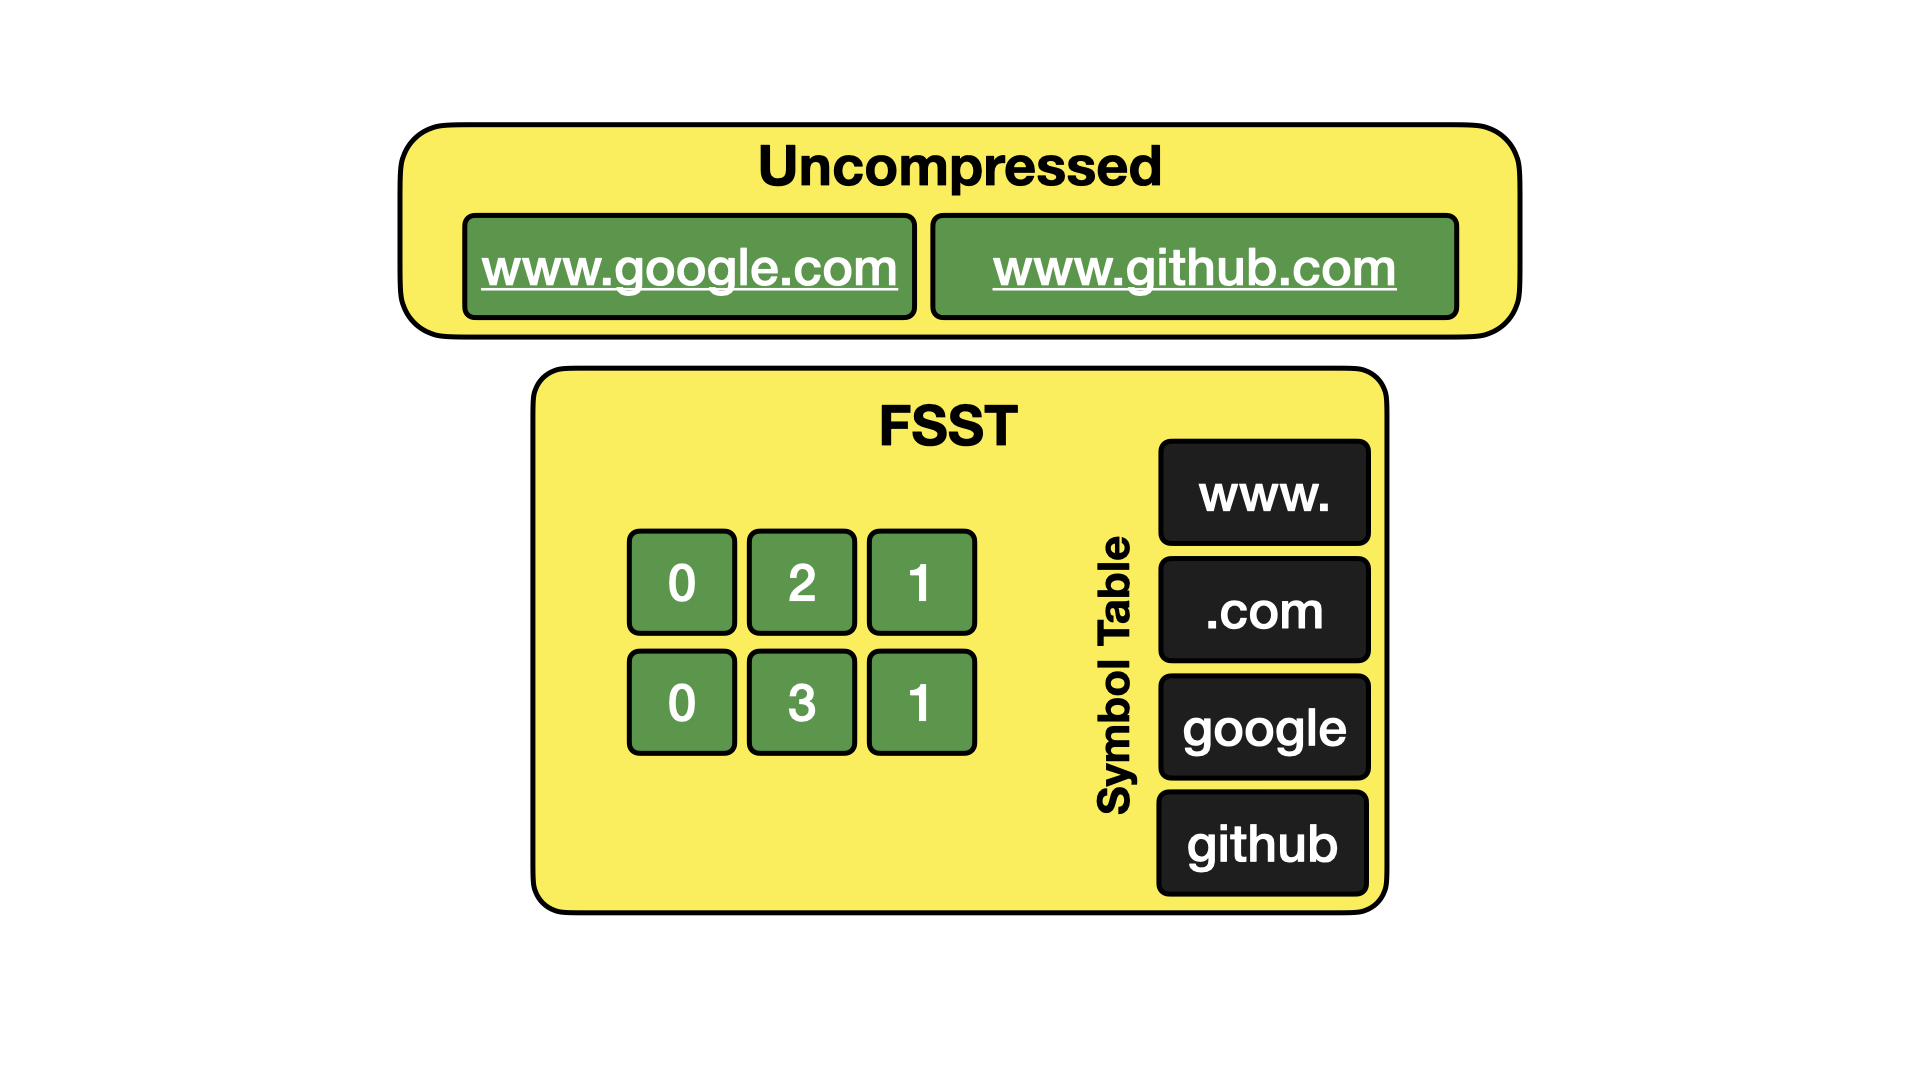
\includegraphics[width=.8\linewidth]{figures/diagrams/10-3_fsst.png}
    \caption[Example of \texttt{FSST} compression]{Example of \texttt{FSST} compression \cite{Raasveldt_2022}}
    \label{fig:fsst}
\end{figure}

Note that in the previous example, the original sequence \texttt{www.google.com} is compressed as \texttt{021}. Where \texttt{0} is the identifier for \texttt{www.}, \texttt{2} identifies \texttt{google} and \texttt{1} stands for \texttt{.com}. As in the case of \textit{run-length encoding} the higher the number of repetitions, the higher the level of compression. In this case, we have successfully represented the initial string, consisting of 14 characters, with a string of only three characters, resulting in a 78\% reduction in size. Although this example is straightforward, it effectively demonstrates the underlying concept of \texttt{FSST}.

One of the greatest strengths of compression in columnar storage lies in the driver's ability to select the optimal algorithm for each scenario. Specifically, in a column-oriented store, we can leverage a variety of compression mechanisms, individually tailored to excel in compressing each column, given that we are dealing with homogeneous data. Conversely, row-oriented stores limit us to a single compression algorithm for the entire dataset. This limitation arises from the heterogeneity of the data, preventing us from employing distinct compression algorithms for each column.

\subsubsection{Data types}

According to what we have seen in the introductory lines, we are going to try and optimize as much as we can the data types that we are going to use for storing the information. For that, we are going to use the smallest data type that can hold the information we are interested in. For example, we are using \texttt{UINTEGER} for storing the IDs of the entities, as they can be represented as numbers. What's more, we are going to use the unsigned representation as we are not interested in negative numbers. This has two main benefits: first, we are going to be able to store larger numbers. To put it into perspective, the maximum value range that can be stored in a \texttt{UINTEGER} is \texttt{4,294,967,295}, whereas the largest number that can be stored in an \texttt{INTEGER} is \texttt{2,147,483,647}. This means that we can handle twice as many positive values with the same number of bits. The same reasoning applies to the rest of the data types that are going to be used. Second, we ensuring e that our data is consistent. This is, we are not going to be able to store negative numbers in a column that is supposed to store positive numbers.

From my perspective, fine-tuning the chosen data types for storing your data makes your repositories more robust. This is because you are ensuring that the data that you are working with is consistent and that you are not wasting any space. This is especially important when dealing with large amounts of data, as the storage footprint can be reduced by a factor of 2. This is the case for this project. At the beginning of it, we were using \texttt{BIGINT} for storing the IDs of the entities. However, we realized that we were wasting half of the space, as the IDs are always positive. For that, we decided to switch to \texttt{UINTEGER}. Summing up, we moved from an 8-byte integer to a 4-byte representation, which means that we were able to store twice as many IDs with the same number of bits. This also leads to fitting more data both in memory and in the cache, which is going to be beneficial for the second part of the tool, where the graph is going to be built.

Regarding the encoding of IDs, we had two main possibilities. First, we could have used the string representation, which is the one that is employed in the JSON dump. However, we decided to go for the numeric representation as it is more compact. This is because the string representation of the IDs is composed of a prefix followed by a sequence of numbers. For example, the string representation of the ID \texttt{Q92743} is \texttt{"Q92743"}, whereas the numeric representation of the same ID is \texttt{92743}. As we are using a \texttt{UINTEGER} for representing the numeric data, only 4 bytes per row are needed. However, a string takes 1 byte per character. Thus, according to the previous example, we would need 6 bytes for encoding the string representation of the ID, while only 4 are required for the numeric representation. In this example, 2 bytes are saved. Note that this scales for even larger IDs.

The problem is that things are not as simple as they seem at first glance. Wikidata IDs not only are numeric identifiers, but they also annotate the type of the item they support: Entities, Properties, Lexemes, Forms and Senses. Thus, we need a way for encoding and decoding this information. For this purpose, what we have done is diving the address space of the IDs into 5 different ranges, one for each type. The ranges have a length of 1 hundred million, except for Forms and Senses, each of them has half that size, which is more than enough for representing the different Wikidata IDs. See the code below for more information.

\begin{code}[The From trait implementation for the ID type]
    \inputminted{rust}{code/listings/10-1_ids.rs}
\end{code}

It is worth mentioning that the most powerful thing about the \texttt{From} \texttt{trait} in Rust is that it allows us to not only convert from one type to another; but in the opposite direction too. This is, it automatically implements the \texttt{Into} \texttt{trait} thanks to the blanket implementation in the standard library. Hence, now we can convert from \texttt{u32} to \texttt{Id} and vice-versa. That is, we can serialize and deserialize the IDs transparently.

\subsubsection{Memory allocator}

A memory allocator is a software component that manages the allocation and deallocation of memory in a program. Its primary goal is to efficiently use available memory by keeping track of allocated and free memory blocks. Allocators work with a memory region called the heap, where objects are dynamically allocated. When a program requests memory, the allocator finds a free block, marks it as allocated, and returns a pointer to the program. Deallocation involves marking the block as free.

Memory allocators can employ various algorithms and data structures to manage memory efficiently. They may use techniques like linked lists, bitmaps, or binary trees to track the state of memory blocks and quickly find free blocks for allocation. Additionally, advanced allocators may employ strategies like caching, thread-specific allocation pools, or memory reuse techniques to optimize performance and reduce overhead.

Different programming languages and platforms often provide default memory allocators, but developers can also choose alternative allocators, such as \texttt{Jemalloc}, for specific optimizations or requirements. By selecting an appropriate memory allocator, developers can improve memory usage, minimize fragmentation, enhance performance, and cater to the specific needs of their applications.

\texttt{Jemalloc} is a memory allocator that can be used in Rust binary projects to optimize memory management and improve application performance. When a program allocates and deallocates memory frequently, the default memory allocator in Rust (system allocator) can introduce overhead due to its design choices and trade-offs, as it is optimized for general-purpose use and targets several different platforms and environments. However, \texttt{Jemalloc} is a specialized allocator that aims for reducing memory fragmentation. When memory allocation and deallocation are frequent, small gaps tend to form between allocated memory blocks. These gaps are called fragmentation and can lead to inefficient memory usage. Note that in the context of Big data applications, efficient memory management may improve the performance of the solution by orders of magnitude. \texttt{Jemalloc} uses a technique called \textit{arena-based memory allocation} to reduce fragmentation and improve performance. It also uses a \textit{thread-specific caching} strategy to reduce the overhead of synchronization and improve performance in multi-threaded applications. As we will see in the next chapter, one of the main optimizations that we will implement is writing our solution in a multi-threaded fashion. Thus, using \texttt{Jemalloc} is going to be beneficial for us. Lastly, note that \texttt{Jemalloc} is a platform-specific allocator, which means that it is only available on Linux and macOS. However, this allows it to use platform-specific features to improve performance.

For us to use \texttt{Jemalloc}, we need to add the following lines to the \texttt{Cargo.toml} file.

\begin{code}[The Cargo.toml file for using Jemalloc]
    \inputminted{toml}{code/listings/10-2_cargo.toml}
\end{code}

What's more, we need to use it as the default allocator for our application. For this, we need to add the following lines to the \texttt{main.rs} file. Recall that the memory allocator should be set in the main function of the application before any other code is executed. This is because the allocator is a global resource, and it is not possible to change it once it has been set. Note that in the case of libraries, changing the allocator won't have any impact, as it is the responsibility of the application to do so.

\begin{code}[The main.rs file for using Jemalloc]
    \inputminted{rust}{code/listings/10-3_main.rs}
\end{code}

\subsubsection{Compiler options}

During the development stage, Rust applications are constructed using the \texttt{dev} flag, which compiles the program without applying any optimizations. By default, the \texttt{opt-level} is set to 0 in order to facilitate easy debugging. The compilation process focuses on detecting potential panics or errors during execution. However, when preparing the tool for deployment, it is recommended to utilize the \texttt{release} profile, which leverages maximum optimization. The \texttt{opt-level} is set to 3 by default, enabling beneficial optimizations. Functions are rewritten to execute faster, incorporating techniques like inlining that make them harder to debug. Additionally, the \texttt{LTO} (Link Time Optimization) is enabled, allowing the compiler to optimize code across different compilation units. This is particularly significant when working with various modules and crates. By utilizing the \texttt{LTO} build, we aim to discover optimizations that span across different dependencies and crates, although this may result in slower compilation times. The \texttt{Cargo.toml} file specifies the release profile as follows:

\begin{code}[The Cargo.toml file for using the release profile]
    \inputminted{toml}{code/listings/10-4_cargo.toml}
\end{code}

\subsubsection{Targeting the right Platform}

Targeting the right platform in Rust is essential for optimizing performance. By specifically focusing on the platform, you can leverage architecture-specific optimizations, taking advantage of specialized hardware accelerators and maximizing the efficiency of memory management. Rust's compiler offers optimization flags and the ability to link with platform-specific libraries, enabling tailored performance enhancements. This approach ensures compatibility with the target platform's operating system, architecture, and hardware configurations, ultimately resulting in improved performance and efficiency for Rust applications. For us to target the right platform, we need to add the following lines to the \texttt{.cargo/config} file.

\begin{code}[The .cargo/config file for targeting the right platform]
    \inputminted{toml}{code/listings/10-5_config}
\end{code}

\subsection{Quality assurance}

In the following subsections, we are going to discuss the different quality assurance mechanisms that are going to be used for the development of the tool. The idea is to ensure that it is robust and that can be used in production environments. For that, we are going to use a combination of different techniques, such as version control, documentation, testing, continuous integration and continuous deployment. Note that the tool is going to be open-source, which means that the community will be able to contribute to the project. This is going to be beneficial for it as it will allow us to build a more robust tool, as third parties can examine the product we ship. Lastly, note that we are going to use this same methodology for the development of the other tools that are going developed in this thesis.

\subsubsection{Version control}

Recall that we are building an open-source solution. For this, we are going to use Git as our version control system. The idea is to use GitHub as our remote repository. This will allow us to have a public warehouse where the community can contribute to the project. Moreover, we are going to use Git tags for the versioning, letting us have a clear understanding of the different versions of the tool. For instance, we are using the \texttt{v0.0.1} tag for the first version. Subsequent versions will be annotated with a \texttt{v0.0.x} tag. What's more, for the sake of simplicity, we are going to use \textit{stable mainline} as our branching strategy for the development of the tool. This means that we are going to have a \texttt{main} branch where the latest stable version is going to be stored. The idea is to have a \texttt{dev} branch where most of the development process is going to take place. Once we have a stable version, we will merge it into the \texttt{main} branch. Note that this is a simple branching strategy that will work just fine for the development of this project as I am the sole developer. However, for larger projects, a more complex branching strategy should be considered.

\subsubsection{Documentation}

Having that said, writing good documentation is essential for the development of a robust project. For that, we are going to use Rust's documentation tool, namely, \texttt{rustdoc}. The idea is to document the different \texttt{functions}, \texttt{structs}, \texttt{traits} and \texttt{modules} of the tool so that the community can have a clear understanding of its API. Moreover, we are going to use \texttt{rustdoc}'s \texttt{doc-tests} feature for writing tests in the documentation. Putting this all together, the whole documentation will be deployed to \texttt{docs-rs}\footnote{\url{https://docs.rs/wikidata-rs/latest/wikidata_rs/}}.

\subsubsection{Testing}

The idea is to have a robust tool that can be used in production environments. For that, we are going to use Rust's testing framework, namely, \texttt{cargo test}. The idea is to write unit tests for the different functions of the tool. Something neat about \textit{unit testing} in Rust is that it encourages developers to write tests in the same file\footnote{\url{https://github.com/angelip2303/pregel-rs/blob/main/src/pregel.rs\#L873}} as the code. This is a good practice as it allows us to have a clear understanding of the different tests that are being run.

\subsubsection{Continuous integration and continuous deployment}

The result of combining the previous techniques is a robust tool that can be used in production environments. However, we are going to take it one step further by using continuous integration and continuous deployment. The idea is to make use of GitHub Actions. This is, having an Action that will run the tests of the tool every time a new commit is pushed to the repository's \texttt{main} branch. This will allow us to have a clear understanding of the state of the tool. Moreover, we are going to have another GitHub Action that will be in charge of deploying the tool to the \texttt{crates.io}\footnote{\url{https://crates.io}} platform so that other developers can use it in their projects.

\subsection{User manual}

\subsubsection{Installation}

Make sure that you install the latest stable version of Rust\footnote{\url{https://www.rust-lang.org/}}; that is, as of May 5th, version 1.69 or later, then run:

\begin{minted}{shell-session}
$ cargo install wd2duckdb
\end{minted}

This will compile \texttt{wd2duckdb} for your native architecture, increasing the performance. Recall the optimizations that we have discussed in the previous section. However, if you want to compile it for a different architecture, you can use the \texttt{--target} flag.

\subsubsection{Usage}

Several command-line options are available to customize the behavior of \texttt{wd2duckdb}. The following is a list of the most important ones:

\begin{enumerate}
    \item \texttt{--json}: The path to the \texttt{.json} file that contains the Wikidata dump. This is a required argument.
    \item \texttt{--database}: The path to the DuckDB database file. This is a required argument.
\end{enumerate}

The following is an example of how to use the tool:

\begin{minted}{shell-session}
$ wd2duckdb --json <JSON_FILE> --database <DUCKDB_FILE>
\end{minted}

Use \texttt{-} as \texttt{<JSON\_FILE>} to read from standard input instead of from a file. This makes it possible to build a pipeline that processes JSON data as it is being decompressed, without having to decompress the full dump to disk. In the case of a \texttt{.bz2} file, you can use the following instruction:

\begin{minted}{shell-session}
$ bzcat latest-all.json.bz2 | wd2duckdb --json - --database <DUCKDB_FILE>
\end{minted}

In case of a \texttt{.gz} compressed file, the following is required:

\begin{minted}{shell-session}
$ gunzip latest-all.json.gz | wd2duckdb --json - --database <DUCKDB_FILE>
\end{minted}

In case you want to write changes directly to the standard output; that is, without creating a file for the uncompressed \texttt{.json}, you can do the following. Note the use of the \texttt{-c} flag in \texttt{gunzip}:

\begin{minted}{shell-session}
$ gunzip -c latest-all.json.gz | wd2duckdb --json - --database <DUCKDB_FILE>
\end{minted}

If you are working with large dumps where the uncompressed \texttt{.json} file size is in the order of \texttt{Terabytes}, it is best to choose the last option. The \texttt{.duckdb} file, which is more memory-efficient, may thus be created immediately. This is because the \texttt{.json} file is not stored in memory, but rather, it is streamed from the standard input.

\subsection{Known limitations}

During the development of our tool, we encountered a limitation related to the \texttt{wikidata}\footnote{\url{https://crates.io/crates/wikidata}} library, which cannot parse JSON dumps before 2017-08-21. This limitation is shared by other tools aiming to import Wikidata dumps\footnote{\url{https://github.com/usc-isi-i2/kgtk/issues/108}}, as mentioned in an issue reported on GitHub. Although the specific reasons for this limitation are not well-documented in Wikidata's developer portal, we have found some clues that may provide insights into the possible cause\footnote{\url{https://github.com/usc-isi-i2/kgtk/issues/272\#issuecomment-748350311}}. The limitation arises from the way references to properties and values are serialized in the dumps. Recall figure \ref{fig:wikibaseStatement}, where we can see that the Statement has a \texttt{mainSnak}, which is the main claim of the statement. Before the mentioned date, the referencing was done using only the numeric identifier (\texttt{numeric-id}) instead of the full identifier expected by the library. For example, the property \texttt{P31} was referenced as \texttt{\{numeric-id: 31\}} instead of \texttt{\{numeric-id: 31, id: "P31"\}}. Hence, the library fails to parse the Wikidata entities. Even if we will continue monitoring the development of the \texttt{wikidata} library to see if this issue is resolved in future updates, fixing it ourselves is challenging and not a priority for our tool's development at the moment, as we can work with dumps from 2017-08-21 onwards.